\chapter{Web Technologies}
\label{chap:WebTechnologies}

\section{HyperText Markup Language (HTML)}
\label{sec:HTML}

HTML is a document markup language for documents which are meant to be displayed in web browsers.
The original proposal and implementation in 1989 came from Tim Berners-Lee who was a contractor at CERN at the time \parencite{TBLProposal}.
Over the years, the standard has been developed by a range of different entities like the CERN and the Internet Engineering Task Force (IETF). 
Nowadays, HTML exists as a continuously evolving living standard without specific version releases which is maintained by the Web Hypertext Application Technology Working Group (WHATWG) and the World Wide Web Consortium (W3C) \parencite{HTML}.

The primary purpose of HTML is to define the content and structure of web pages.
This is achieved with the help of HTML elements, which are composed in a hierarchical tree structure and define modular pieces of content which can be interpreted by web browsers.
A strong pillar of HTML's design is extensibility and there are multiple mechanisms in place to ensure applicability to a vast range of use cases.
These mechanisms include:

\begin{itemize}
\item Specifying classes of elements using the \attrname{class} attribute.
This effectively creates custom elements while still basing them on the most related, already existing elements.

\item Using \attrname{data-*} attributes to decorate elements with additional data which can be used by scripts.
The HTML standard guarantees that these attributes are ignored by browsers.

\item Embedding custom data using \elname{<script type="">} elements which can be accessed by scripts.
\end{itemize}


\section{Cascading Style Sheets (CSS)}
\label{sec:CSS}

This section is meant to give an overview and reiterate over the CSS concepts which are important in the context of this thesis.
In particular, the history of CSS is briefly summarized, a refresher on selectors and cascades is given and the different modules of CSS-based layouting are compared.

Cascading Style Sheets (CSS) is a style sheet language which is used to specify the presentation of HTML documents. 
It can either be embedded directly in HTML documents using \elname{<style>} elements or it can be defined externally and linked into them using \elname{<link>} elements. 
This characteristic of being able to externally describe the presentation of documents yields a lot of flexibility because multiple documents with different content can reuse the same presentation by linking to the same CSS file. 
This solved the problem of having to individually define the presentation of every page with presentation elements like \elname{<strong>} or \elname{<em>}, as was the case in earlier versions of HTML \parencite{HTML32}.

CSS was initially proposed by \cite{CSSProposal} and standardized into CSS1 by the W3C in 1996 \parencite{CSS1}. 
Throughout its history, the adoption of CSS by browser vendors was fraught with complications and even though most major browsers soon supported almost the full CSS standard, their implementations sometimes behaved vastly different from their competitor's. 
This meant that authors of web pages usually had to resort to workarounds and provide different style sheets for different browsers. 
In recent years, CSS specifications have become much more detailed \parencite{CSS21} and browser implementations have become more stable with fewer inconsistencies. 
It has therefore become much rarer that browser-specific workarounds need to be applied, which
drastically improves the development experience.

A CSS style sheet contains a collection of rules and each rule consists of a selector and a block of style declarations. 
Selectors are defined in a custom syntax and are used to match HTML elements. 
All elements which are matched by the selector of a rule will have the rule's style declarations applied to them. 
The selector syntax is fairly simple when merely selecting elements of a certain type, but it also provides the means for selecting elements based on their contexts or attributes. 
For a summary of the CSS 2.1 selector syntax, see Table \ref{tab:CSSSelectorSyntax}.

\begin{table}[tp]
\tablestretch
\rowcolors{2}{}{tablerowcolour}
\centering
\begin{tabularx}{\linewidth}{>{\kern-\tabcolsep}lX<{\kern-\tabcolsep}}
\toprule
Pattern & Matches \\
\midrule
\pattname{*}      & Any element. \\
\pattname{E}      & Elements of type E. \\
\pattname{E F}    & Any element of type F which is a descendant of elements of type E. \\
\pattname{E > F}  & Any element of type F which is a direct descendant of elements of type E. \\
\pattname{E + F}  & Any element of type F which is a directly preceded by a sibling element of type E. \\
\pattname{E:P}    & Elements of type E which also have the pseudo class P. \\
\pattname{.C}     & Elements which have the class  C. \\
\pattname{#I}     & Elements which have the ID I. \\
\pattname{[A]}    & Elements which have an attribute A. \\
\pattname{[A=V]}  & Elements which have an attribute A with a value of V. \\
\pattname{S1, S2} & Elements which match either the selector S1 or the selector S2. \\
\bottomrule
\end{tabularx}
\caption[CSS Selector Syntax]{
  A summary of the CSS 2.1 selector syntax.
  \imgcredit{Table created by the author of this thesis with data from \cite{CSS21}}
}
\label{tab:CSSSelectorSyntax}
\end{table}

Another important characteristic of CSS is the cascading of styles. 
There's a lot of depth to how the final style of an element is calculated and \cite{CSS21} should be consulted for detailed notes on this topic. 
The most important thing to state in the context of this work, is that styles can be overwritten. 
When multiple rules match an element and define different values for the same style property, the values of the rule with higher specificity will be applied. 
If multiple rules have the same specificity, the one defined last in the document tree will overwrite all previous ones.

\subsection{Box Layout}
\label{sec:BoxLayout}

All elements in an HTML document are laid out as boxes. 
This is defined as the CSS box model which means that every element is wrapped in a rectangular box and every box is described by its content and the optional surrounding margin, border and padding areas.
Margins are used to specify the invisible spacing between boxes, whereas the border is meant as a visible containment around the content of a box and the padding describes the invisible spacing between the content and the border. 
A visual representation of these properties can be seen in Figure \ref{fig:BoxModel}.

\begin{figure}[tp]
\centering
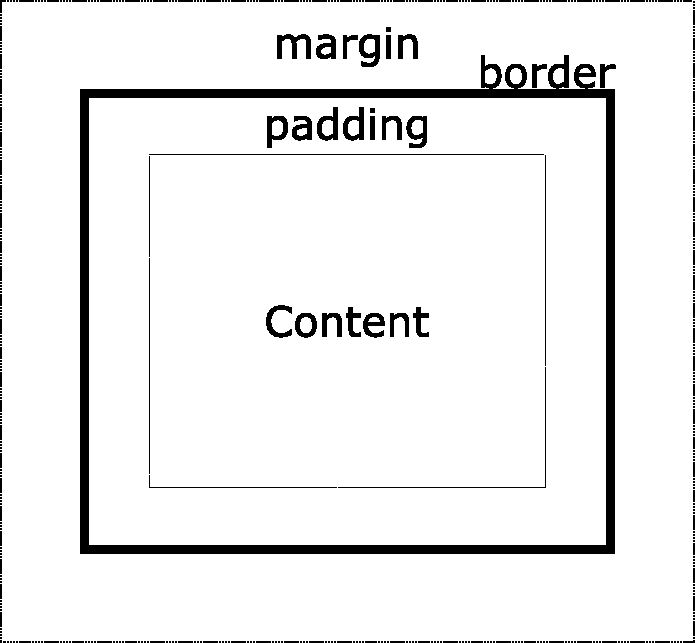
\includegraphics[keepaspectratio,width=\linewidth,height=\fullh / 4]{diagrams/box-model.pdf}
\caption[CSS Box Model]{
  The CSS box model is used to define the properties of boxes which wrap around HTML elements.
  \imgcredit{Image drawn by the author of this thesis.}
}
\label{fig:BoxModel}
\end{figure}

In early versions of CSS, before the introduction of the Flexible Box (Flexbox) layout module \parencite{CSSFlexboxFirstDraft}, the box model was the only way to lay out elements. 
Style sheet authors had to meticulously define margins of elements and their relative (or absolute) positions in the document tree. 
The responsive capabilities of this kind of layouting are very limited because different configurations for varying screen sizes have to be specified manually using media queries.
More complex features, like the filling of available space, require manual implementations via scripting.

\subsection{Flexible Box (Flexbox) Layout }
\label{sec:Flexbox}

Even though the first draft of the Flexbox layout module was already published in 2009 \parencite{CSSFlexboxFirstDraft}, implementations by browser vendors have been a slow and bug ridden process \parencite{CanIUseCSSFlexbox} which held back adoption by users for the first couple of years after its inception. 
Over the past few years, partly through the deprecation of Internet Explorer \parencite{IEDeprecation}, all major browser implementations of current Flexbox standards \parencite{CSSFlexbox} have reached maturity and, in most cases, fallback styling is not necessary anymore.

Flexbox is a mechanism for one-dimensionally laying out elements in either rows or columns. 
This one-dimensionality is what separates it from grid-based layouting, which is inherently two-dimensional. 
Flexbox layouting can be enabled for child elements via setting the \cssname{display:flex} property on a container element. 
The direction of the layout can then be specified using the \cssname{flex-direction} property which can be set to either \cssname{row} or \cssname{column}.

The items inside a Flexbox container can have either a fixed or a relative size. 
When items should be sized relative to the size of their containers, the proportions of how the available space should be divided can be controlled using ratios. 
These ratios can be set on item elements via the \cssname{flex} property.

Another important feature of Flexbox layouting is the controllable spacing of items which can be specified separately for both the main and the cross axis of the layout. 
Spacing along the main axis can be configured with the \cssname{justify-content} property which can take a number of different values which are demonstrated in Figure \ref{fig:FlexboxJustifyContent}. 
The property which controls alignment of items on the cross axis is either the \cssname{align-items} property on container elements or the \cssname{align-self} property on the items themselves.

\begin{figure}[tp]
\centering
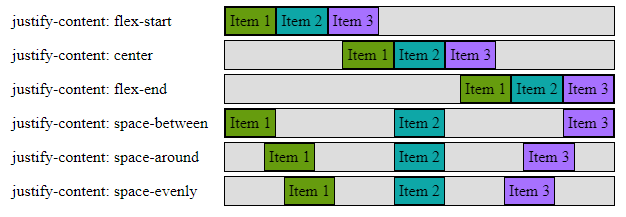
\includegraphics[keepaspectratio,width=\linewidth,height=\fullh / 3]{images/flexbox-justify-content.png}
\caption[Flexbox Justify Content Property]{
  The \cssname{justify-content} property is used to distribute items along the main axis of a Flexbox container. 
  \imgcredit{Image created by the author of this thesis.}
}
\label{fig:FlexboxJustifyContent}
\end{figure}

This section only graced the surface of what is possible with the Flexbox layout module. 
Those properties which were discussed, were only discussed in a very broad sense and there are many useful properties like \cssname{flex-grow}, \cssname{flex-shrink} or \cssname{flex-wrap} which were not included in this overview. 
For a more detailed look at this topic it is recommended to review \cite{CSSFlexbox}.

\subsection{Grid Layout}
\label{sec:Grid}

Similar to the previous section about Flexbox layout, the goal of this section is not to be a comprehensive guide on the CSS Grid layout module but to provide a rough overview over its general characteristics. 
For more detailed information, other sources like \cite{GridLayoutInCSS} and \cite{CSSGrid} are recommended.

The initial proposal of the CSS Grid layout module has already been published in 2011 \parencite{CSSGridFirstDraft} and it has been further refined over the years. 
At the time of writing, even though it still exists as merely a candidate recommendation for standardization \parencite{CSSGrid}, many browsers have already adopted it. 
The history of browser adoption has been, similar o the one of Flexbox layout, filled with inconsistencies and bugs. 
However, browser support has been considered stable and safe to use since 2017 when Chrome, Firefox, Safari and Edge removed the need for vendor prefixes and the deprecation of IE was announced \parencite{CanIUseCSSGrid}.

The Grid layout module defines laying out elements in a two-dimensional grid, which differences it from the one-dimensional layouting which can be achieved with a Flexbox layout. 
Grid layouting of elements can be enabled by setting the \cssname{display:grid} property on their container. 
The grid in which items shall be laid out is then defined using the \cssname{grid-template-rows} and \cssname{grid-template-columns} properties. 
There also exists the \cssname{grid-template} property, which can be used as a shorthand to simultaneously specify both rows and columns of a grid.

Item elements need to specify the cell of the grid into which they shall be positioned. 
This is done with the \cssname{grid-row} and \cssname{grid-column} properties, which take the corresponding row and column indices as values. 
Items can also be configured to span multiple cells by not only specifying single indices but whole index ranges as the values of those properties.

Every cell in a grid can also be assigned a specific name via the \cssname{grid-template-areas} property on the grid container element. 
The items within the grid can then position themselves in specifically named grid cells using the \cssname{grid-area} property instead of directly setting the row and column indices. 
The benefit of positioning items this way is that the structure of the grid can freely be changed without having to respecify the cells in which items belong. 
As long as the new layout still specifies the same names of cells somewhere in the grid, the items will be automatically placed at their new positions.

There are also properties which allow to control the layout of items within grid cells and the layout of grid cells themselves. 
Similar to how it is described in Section \ref{sec:Flexbox}, this can be configured with the \cssname{align-items} and \cssname{justify-items} properties for laying out within grid cells, and the \cssname{align-content} and \cssname{justify-content} properties for laying out the grid cells themselves. 
The latter \cssname{*-content} properties only make sense when the cells do not cover the full area of the grid. 
For a visual comparison between the \cssname{*-items} and \cssname{*-content} properties, see Figure \ref{fig:GridLayoutProperties}.

\begin{figure}[tp]
\centering
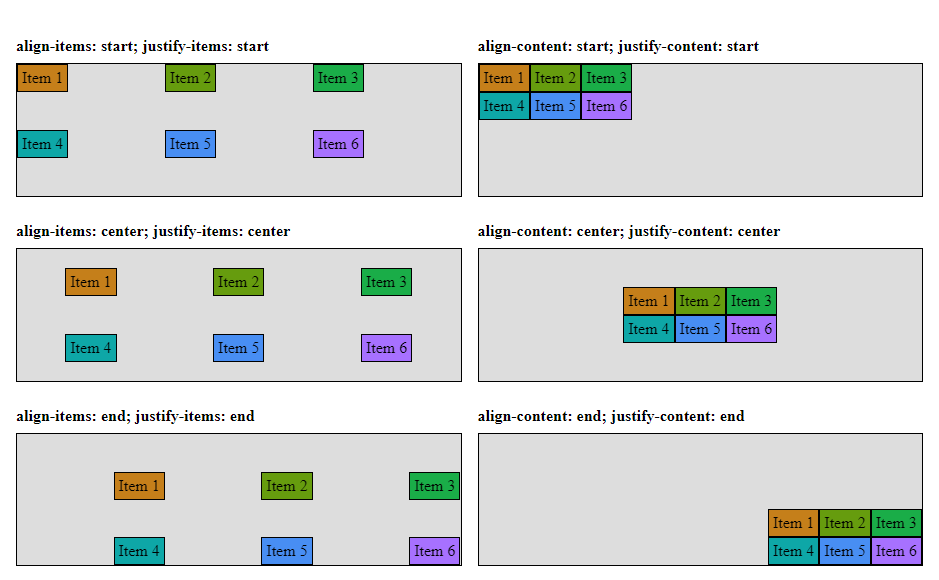
\includegraphics[keepaspectratio,width=\linewidth,height=\fullh / 2]{images/grid-layout-properties.png}
\caption[Grid Layout Property Comparision]{
  The \cssname{*-items} properties are used to lay out items within their grid cells, whereas the \cssname{*-content} properties are used to lay out the grid cells themselves. 
  \imgcredit{Image created by the author of this thesis.}
}
\label{fig:GridLayoutProperties}
\end{figure}

There is a large overlap between the CSS Grid and Flexbox layout modules and, at first sight, it seems like Grid layout supersedes Flexbox layout because everything which can be done using Flexbox layout can also be done with Grid layout. 
While that is true, the inherent difference in dimensionality and the resulting syntactical characteristics lead to better suitability of one technology over the other, depending on the situational requirements. 
As a general rule \parencite{CSSGridVsFlexbox}, top-level layouts which require two-dimensional positioning of elements are usually implemented using a Grid layout, whereas low-level layouts which merely need laying out on a one-dimensional axis are more expressively described using a Flexbox layout.

\section{JavaScript (JS)}
\label{sec:JS}

JavaScript (JS) is one of the three core technologies of the web: HTML for content, CSS for presentation and JS for behavior. 
the goal of this section is to briefly summarize JS, its history and the specific Web APIs which are relevant for this work.

JavaScript is a client-side scripting language which requires an engine which interprets it. 
These engines are usually provided by browsers, but there are also standalone engines, like NodeJS \parencite{NodeJS}, available. 
JavaScript is a multi-paradigm language which supports event-driven, as well as functional and imperative programming.
Undoubtedly influenced by the popularity of the web, JavaScript is currently the most used programming language worldwide \parencite{StatisticProgrammingLanguageUsage}.

It has initially been created by Netscape in 1995 \parencite{JSFirstRelease}.
Before that, websites were only able to display static content, which drastically limited the usefulness of the web. 
Seemingly, Microsoft saw JavaScript as a potentially revolutionary development because they reverse-engineered the implementation of Netscape and published their own version of the language for Internet Explorer in 1996 \parencite{JSIERelease}. 
Both implementations were noticeably different from one another and the uncontested monopoly of the Internet Explorer \parencite{BrowserMarketShareEarly} held back standardization efforts undertaken by Netscape \parencite{ECMAScript1}. 
When Firefox was released in 2004 \parencite{FirefoxFirstRelease} and Chrome in 2008 \parencite{ChromeFirstRelease}, they quickly gained a considerable share of the market \parencite{BrowserMarketShare} (see Figure \ref{fig:BrowserMarketShare}).
Driven by this new market segmentation, all major browser vendors collaborated on the standardization of JavaScript as ECMAScript 5 in 2009 \parencite{ECMAScript5}. 
Since then, JavaScript has been continuously developed and its latest, widely support version, ECMAScript 6, has been released in 2015 \parencite{ECMAScript6}.

\begin{figure}[tp]
\centering
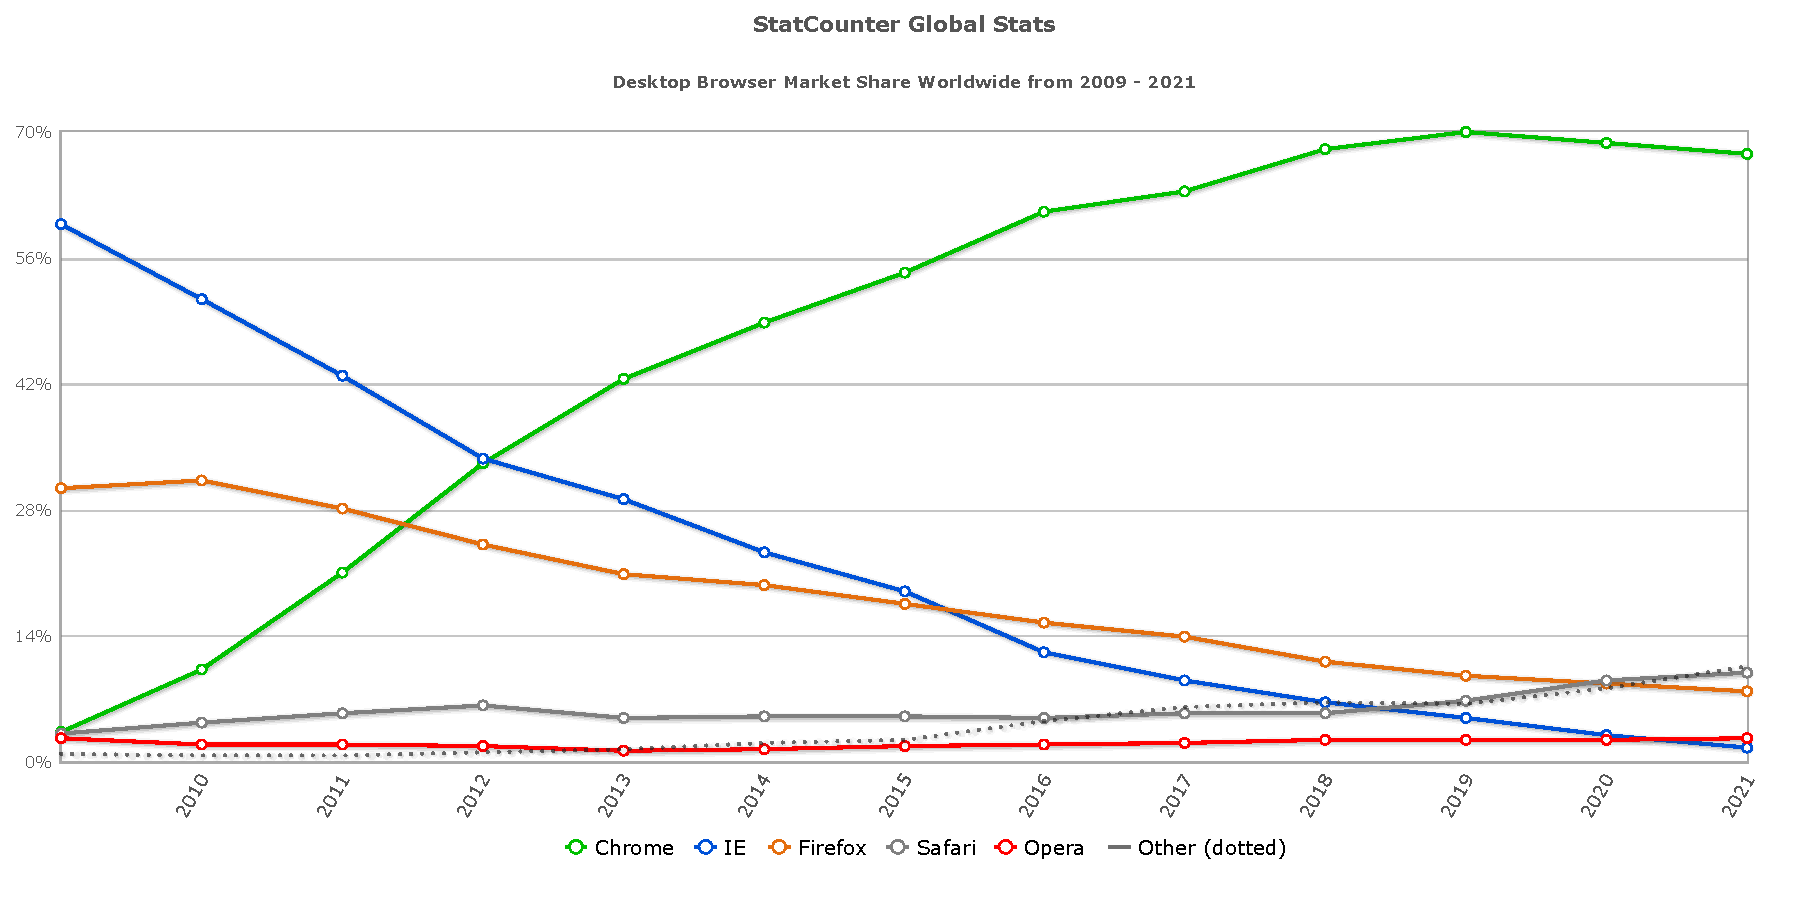
\includegraphics[keepaspectratio,width=\linewidth,height=\fullh / 3]{diagrams/browser-market-share.pdf}
\caption[Desktop Browser Market Share]{
  Since their release, Firefox and Chrome have contested the monopoly of the Internet Explorer and continuously gained more market share. 
  Recently, Chrome seems to be gaining an increasingly strong position within the market. 
  \imgcredit{Image taken from \cite{BrowserMarketShare}}}
\label{fig:BrowserMarketShare}
\end{figure}

RespVis is a browser-based library which is designed to run within the JavaScript engine of a browser. 
Therefore, it builds heavily on widely supported Web APIs which are JavaScript modules which are specifically meant for the development of web pages. 
These Web APIs are standardized by the W3C and each browser has to individually implement them in their JavaScript engine.

The most popular Web API which every web developer is familiar with is the Document Object Model (DOM).
The DOM is the programming interface and data representation of a document. 
Internally, a document is modeled as a tree of objects, where each object corresponds to a specific element in the document hierarchy and its associated data and functions. 
In addition to the querying of elements, the DOM also defines the functionality to mutate them and their attributes, as well as the functionality for handling and dispatching of events. 
It also exposes the mechanism of \modname{MutationObservers}, which are used to observe changes of attribute and children in the document tree. 
The initial publication of the DOM dates back to 1998 \parencite{DOM1} and currently it is maintained as a living standard by the WHATWG \parencite{DOM}.

Another important Web API in the context of this work is the \modname{ResizeObserver} API. 
Its purpose is the ability to observe an element's size and respond to changes, which increases the responsive capabilities of websites. 
Previously, scripts could only respond to changes in the overall viewport size via the \lstinline{resize} event on the \lstinline{window} object, but this meant that changes of an individual element's size through attribute changes could not be detected. 
This limitation is fixed by the \modname{ResizeObserver} API, which is already fully supported by all modern browsers, even though it has so far only been published as an editor's draft \parencite{ResizeObserver}.

\section{TypeScript (TS)}
\label{sec:TS}

TypeScript (TS) is a strongly-typed programming language which is designed as an extension of JavaScript. 
Syntactically, it is a superset of JavaScript which enables the annotation of properties, variables, parameters and return values with types. 
It requires a compiler which transpiles TypeScript code into valid JavaScript code based on specific ECMAScript versions.

Initially, TypeScript has been released by Microsoft in 2012 \parencite{TSFirstRelease} to extend JavaScript with features which were already present in more mature languages, and whose absence in JavaScript caused difficulties when working on larger codebases. 
At the time of TypeScript's initial development, it was used to already be able to use features which would later be offered by ECMAScript 6.
These features included a module system to be able to split source code into reusable chunks and a class system to aid object-oriented development. 
The TypeScript code using these features could then be translated via a compiler into standard-conform JavaScript code, which could be interpreted by JavaScript engines at the time. 
At the time of writing, ECMAScript 6 is already widely supported by all modern browsers and therefore the main benefit of TypeScript over JavaScript resides primarily in the addition of a static type system.

The extension of JavaScript with a type system brings many benefits. 
One such a benefit is the improved tooling which comes with type annotated code. 
Tools will be able to point out errors early during development and assist developers with automated fixes, improved code completion, and code navigation. 
Additionally, studies like \cite{ToTypeOrNotToType} have evaluated software bugs in publicly available codebases and found that 15\% of them could have been prevented with static type checking.

The TypeScript type system has been designed to support the constructs which are possible in JavaScript as completely as possible, which is achieved via structural types and unified object types. 
Another goal has also been to make the type annotation of JavaScript code as effortless as possible to improve adoption by already existing projects. 
This is done by consciously allowing the type system to be statically unsound via gradual typing and also by employing type inference to reduce the amount of necessary annotations. 
The major properties of TypeScript's type system design are summarized in Table \ref{tab:TSTypeSystemDesignProperties}.

\begin{table}[tp]
\tablestretch
\rowcolors{2}{}{tablerowcolour}
\centering
\begin{tabularx}{\linewidth}{>{\kern-\tabcolsep}lX<{\kern-\tabcolsep}}
\toprule
Design Property & Description \\
\midrule
Full erasure         & Types are completely removed by the compiler and therefore there is also no type checking at runtime. \\
Type inference       & A big portion of types can be inferred from usage, which minimizes the number of types which have to be explicitly written. \\
Gradual typing       & Type checking can be selectively prevented by using the dynamic \lstinline{any} type. \\
Structural types     & Types are defined via their structure as opposed to nominal type systems, which define types via their names. This better fits to JavaScript because here, objects are usually custom-built and used based on their shapes. \\
Unified object types & A type can simultaneously describe objects, functions and arrays. These constructs are common in JavaScript and therefore TypeScript needs to enable their typing. \\
\bottomrule
\end{tabularx}
\caption[TypeScript Type System Design Properties]{
  A summary over the major design properties on which TypeScript's type system is built.
  \imgcredit{Table created by the author of this thesis with data from \cite{UnderstandingTS}.}
}
\label{tab:TSTypeSystemDesignProperties}
\end{table}

\section{Web Graphics}
\label{sec:WebGraphics}

Graphics are used as a medium for visual expression to enhance the representation of information on the web. 
There are versatile fields of application like the integration of maps, photographs or charts in a website. 
Multiple complementary technologies exist and each solves particular use cases of web authors. 
The different ways of embedding graphics in a document are raster images, Scalable Vector Graphics (SVG) and through the Canvas API. 
These technologies are described in the following sections.

\subsection{Raster Images}
\label{sec:RasterImages}

Raster images represent graphics as a rectangular, two-dimensional grid of pixels with a fixed size. 
This fixed grid size results in limited scalability and whenever an image is displayed in a different size, visual scaling artifacts will be noticeable as can be seen in Figure \ref{fig:RasterImage}. 
Raster images are either created by image capturing devices or special editing software and saved as binary files in varying formats. 
The most widely used format for raster images is Portable Network Graphics (PNG), which is standardized by the W3C \parencite{PNG} and optimized for usage on the web. 
It features a lossless compression and streaming capabilities, which enable progressive rendering of images while they are loaded.

Raster images are embedded into documents in binary format. 
This means that the contents of the graphic are not accessible in a non-visual representation. 
To make the information accessible to visually impaired people it is required to provide an additional textual description of the graphic's content on the embedding element via the \attrname{alt} and \attrname{longdesc} attributes.

\begin{figure}[tp]
\centering
\subfloat[][]{
\includegraphics{images/circle.png}\label{fig:RasterImage1}}
\subfloat[][]{
\includegraphics[keepaspectratio,width=0.5\linewidth,height=\fullh / 4]{images/circle.png}\label{fig:RasterImage2}}
\caption[Raster Image Scaling]{
  This figure demonstrates the artifacts which occur when scaling raster images to a size which is different from the size they were encoded in.
  \subref{fig:RasterImage1} shows a raster image of a circle in its original size.
  \subref{fig:RasterImage2} shows the same image scaled up considerable. 
  \imgcredit{Image created by the author of this thesis.}
}
\label{fig:RasterImage}
\end{figure}

\subsection{Scalable Vector Graphics (SVG)}
\label{sec:SVG}

Scalable Vector Graphics (SVG) is an XML-based format for vector graphics which describe images as sets of shapes which can be scaled without loss of quality. 
It was initially published by the W3C in 1999 \parencite{SVG1} and the most recent version SVG 1.1 was released in 2011 \parencite{SVG11}. 
SVG files are based on XML and therefore can be created with any text editor, but there is also specialized software available which helps with the composition of more complex images.
A simple example of an SVG document containing a single circle can be seen in Listing \ref{list:SVG} with its visualization being shown in Figure \ref{fig:SVG}. 

\begin{samepage}
\lstinputlisting[%
  float=tp,
  aboveskip=\floatsep,
  belowskip=\floatsep,
  xleftmargin=0cm,              % no extra margins for floats
  xrightmargin=0cm,             % no extra margins for floats
  language=XML,
  basicstyle=\footnotesize\ttfamily,
  frame=shadowbox,
  numbers=left,
  label=list:SVG,
  caption={
    [SVG Document Containing a Circle]%
    A simple SVG document containing a circle element. 
    The visual representation of this document in different sizes is shown in Figure \ref{fig:SVG}
  }
]{listings/circle.svg}
\end{samepage}

\begin{figure}[tp]
\centering
\subfloat[][]{
\includegraphics[keepaspectratio,width=0.05\linewidth,height=\fullh / 4]{images/circle.pdf}}
\subfloat[][]{
\includegraphics[keepaspectratio,width=0.5\linewidth,height=\fullh / 4]{images/circle.pdf}}
\caption[SVG Scaling]{
  SVG documents can be scaled freely without any artifacts occurring. 
  This figure displays the visual representation of the SVG document in Listing \ref{list:SVG} scaled to different sizes. 
  \imgcredit{Image created by the author of this thesis.}
}
\label{fig:SVG}
\end{figure}

The encoding in XML leads to SVG being the best format to represent graphics in terms of accessibility.
Graphics are directly saved in a hierarchical and textual form which describes their shapes and how they are composed. 
In addition to the shapes being inherently accessible, the various elements of an SVG document can be annotated with further information which aids comprehension when consumed in a non-visual way.

SVG files are XML documents whose meta format is described in special SVG namespaces. 
Therefore, the elements of SVG documents can be accessed in scripts via the DOM Web API. 
This means that elements can be completely controlled by scripts, which enables similar levels of interactivity than for HTML documents.

The most widely supported way of styling SVG elements is via attributes, which is supported by every software dealing with SVG files. 
However, the specification aims for maximum compatibility with HTML, and therefore it is also possible to use CSS to style and animate SVG elements when they are rendered in a browser. 
Using CSS to separate presentation from content has many benefits which were already described in Section \ref{sec:CSS}.
Unfortunately it is not possible to style every SVG attribute with CSS because only the so-called presentation attributes like \cssname{fill} and \cssname{stroke-width} are available in CSS. 
These presentation attributes are taxonomically listed in the SVG specification \parencite{SVG11} and will be extended by additional attributes like \cssname{x}, \cssname{y}, \cssname{width} and \cssname{height} in upcoming releases \parencite{SVG2}.

\subsection{Canvas (2D)}
\label{sec:Canvas2D}

The canvas element has been introduced in HTML5 \parencite{HTML} and is used to define a two-dimensional, rectangular region in a document which can be drawn into by scripts.
Even though the rendering of dynamic graphics as canvas elements is faster than representing them as SVG documents, their use is explicitly discouraged by the WHATWG when another suitable representation is possible.
The reasons for this are that canvas elements are not compatible with other web technologies like CSS or the DOM Web API and because the resulting rendering as a raster image provides only very limited possibilities for accessibility.

Rendering is programmed via a low-level API which is provided by the rendering context of a particular canvas. 
The type of render context depends on the context mode of a canvas with the two most significant ones being \lstinline{2d} and \lstinline{webgl}. 
A two-dimensional render context is created for canvases which have the \lstinline{2d} context mode set on them.
It enables platform-independent rendering via a software renderer, whose API is standardized directly in the canvas specification. 
An example of an HTML document containing two differently sized canvases into which responsive circles are drawn using a two-dimensional rendering context can be seen in Listing \ref{list:Canvas} with the corresponding visualization displayed in Figure \ref{fig:Canvas}.

\begin{samepage}
\lstinputlisting[%
  float=tp,
  aboveskip=\floatsep,
  belowskip=\floatsep,
  xleftmargin=0cm,              % no extra margins for floats
  xrightmargin=0cm,             % no extra margins for floats
  basicstyle=\footnotesize\ttfamily,
  frame=shadowbox,
  numbers=left,
  label=list:Canvas,
  caption={
    [Canvas With Responsive Circles]%
    A basic HTML document containing two canvases of different sizes which render circles relative to the canvas size. 
    The visual representation of this document is shown in Figure \ref{fig:Canvas}.
  }
]{listings/canvas.html}
\end{samepage}

\begin{figure}[tp]
\centering
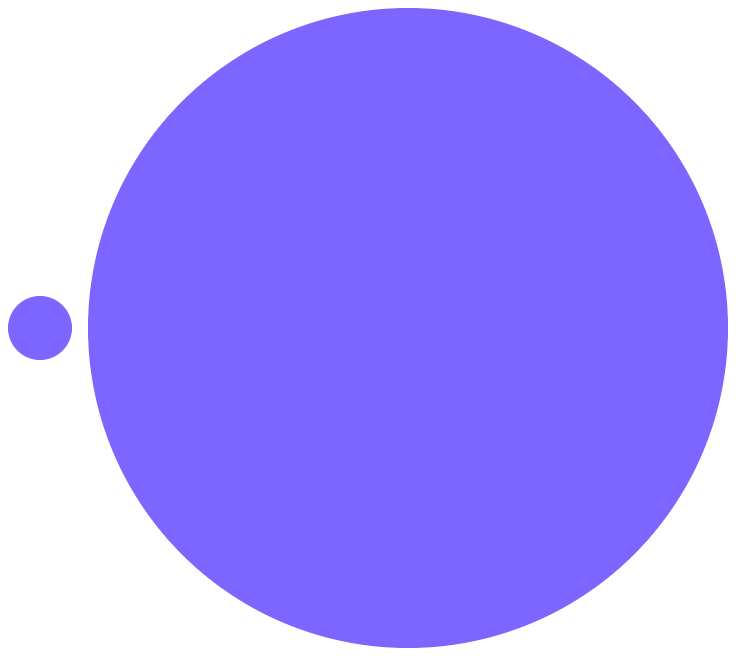
\includegraphics[keepaspectratio,width=\linewidth,height=\fullh / 4]{images/canvas.png}
\caption[Canvas With Responsive Circles]{
  Responsive rendering of graphics inside canvas elements has to be implemented manually by calculating everything as ratios of the canvas' dimensions. 
  This figure represents the visual representation of the canvas example in Listing \ref{list:Canvas}. 
  \imgcredit{Image created by the author of this thesis.}
}
\label{fig:Canvas}
\end{figure}

\subsection{Canvas (WebGL)}
\label{sec:CanvasWebGL}

A three-dimensional render context is created for canvas elements which have their context mode set to \lstinline{webgl} .
Three-dimensional rendering is even faster than two-dimensional rendering via the platform-independent software renderer provided for two-dimensional render contexts.
The reason for this is that three-dimensional rendering is performed via a hardware-accelerated WebGL renderer.
Even though the API of the WebGL renderer is also standardized \parencite{WebGL}, the availability of individual features depends on the client's hardware.
It is therefore recommendable to only use three-dimensional rendering when the requirements do not allow for any of the alternatives.

\section{Layout Engines}

A layout engine is used to calculate the boundary coordinates of visual components based on some form of input components which are annotated with layout constraints. 
These layout constraints describe the size and position of components and their relationships between each other in a syntax which is understood by the layout engine. 
For browser-based layout engines these input components are normally declared as HTML documents which are constrained using CSS. 
More low-level layout engines require custom formats, which usually involve a hierarchy of objects which are constrained using specific properties. 
The most relevant layout engines in the context of this work are summarized in the following sections.

\subsection{Browser Engines}
\label{sec:BrowserEngines}

The purpose of a browser engine is to transform documents including their additional resources, like CSS, into visual representations. 
A browser engine is a core component of every web browser, and it is responsible for laying out elements and rendering them. 
The terminology of browser engines is very vague with them sometimes also being referred to as layout or render engines. 
Theoretically, the layout and render processes could be separated into different components, but in practice they are tightly-coupled into a combined component, which will be referred to as a browser engine in this work. 
Some notable browser engines are WebKit \parencite{WebKit}, Blink \parencite{Blink} and Gecko \parencite{Gecko}.

In a browser engine the layout of elements is constrained with CSS, which gives website authors a lot of flexibility as already described in Section \ref{sec:CSS}. 
They are offered a range of mechanisms to precisely control the layout of elements, like the flexible box and grid layout modules, which do not have to be applied exclusively but can also be used in combination. 

The layout module of a browser engine can only be invoked directly by browsers to position HTML elements in actively rendered documents. 
To use it for calculating layouts of non-HTML constructs, they must be replicated in active documents, so they can be parsed, laid out and rendered by the browser engine. 
These replicated constructs do not have to be visible, and they could also be removed from the document after the layout has been acquired, meaning they do not need to be noticeable at all. 
A strong limitation of using browser engines to calculate layouts is that it requires a browser runtime to work and, even though there are solutions like Electron available which enable development of desktop applications using web technologies, this limitation forces applications into a very specific stack of technologies. 

\subsection{Yoga}
\label{sec:Yoga}

Yoga \parencite{Yoga} is a layout engine which enables the computation of layouts which are constrained using the grammar defined in the Flexbox layout module (see Section \ref{sec:Flexbox}). 
It is maintained by Facebook as an open-source project since 2016 \parencite{YogaRelease} with the goal of providing a small and high-performance library which can be used across all platforms. 
This is achieved through the implementation being programmed in the C/C++ programming language, which works on a myriad of devices, with bindings available for other platforms like JavaScript, Android and iOS.
Yoga has been very well adopted and is used to perform layouting in major frameworks such as React Native \parencite{ReactNative}, Litho \parencite{Litho} and ComponentKit \parencite{ComponentKit}.

\subsection{FaberJS}
\label{sec:FaberJS}

FaberJS \parencite{FaberJS} is a layout engine which is very similar to the Yoga layout engine in the fact that it enables the computation of layouts for constructs other than HTML documents, using a layout grammar which has originally been created for CSS. 
In contrast to Yoga, which is used to create one-dimensional layouts using the Flexbox layout grammar, FaberJS implements a two-dimensional layout algorithm which is built on the grammar of the Grid layout module (see Section \ref{sec:Grid}). 
This inherently two-dimensional approach to layouting is more suited to information visualization than trying to achieve two-dimensionality using a one-dimensional one. 
FaberJS is an open-source JavaScript project and has been developed since 2019 by Idera, Inc.
Even though the layouts it computes are constrained with the grid layout grammar, it only supports a subset of all the functionalities defined in the original CSS module. 
Some examples of missing functionalities include missing support for margins, gaps and the \cssname{*-content} and \cssname{grid-auto-*} properties. 
Working around the limitations caused by these missing features is not trivial, and it seems unlikely that support for them will be added by the FaberJS maintainers in the near future because, at the time of writing, the project has not been updated in nearly two years. 

\section{Responsive Web Design}
\label{sec:RWD}

Influenced by the increasing use of mobile devices and their vastly varying screen sizes, responsive web design has established itself as the predominant way of designing web pages. 
The core idea of responsive web design is that instead of designing pages for different types of devices, website authors create a single design for a page which adapts to the characteristics of the consuming device. 
The term "Responsive Web Design" has been defined by \cite{ResponsiveWebDesign} where the author differentiates between flexible and responsive web designs. 
It states that a flexible web design, which merely fluidly scales blocks of content to make them fit into the width of a browser window, is not enough to provide a good experience for users. 
Such designs will work well enough for similarly sized viewports to the one they were created for, but they will lead to noticeable artifacts on lower resolutions. 
These problems can be avoided by positioning the individual components of a page in a manner which provides them with enough space to render correctly.
This can be achieved by using CSS media queries to adapt the overall layout of a page to the dimensions of the consuming device. 
Another crucial part of responsive web design is to support the different modes of interaction inherent to the various types of devices used to access the web. 
Desktop users might access a website using a mouse, mobile device users are usually interacting via touchscreens, and yet others might consume a page in a purely textual form with a screen reader which requires interaction via keyboard. 
It is one of the mantras of responsive web design to provide smooth and complete access to information to all users, regardless of the device they are using. 